%\newpage
\section{Patient Details}


% View patient details
\subsection{View patient details}
\textbf{Description:}
This allows the administrator to view the details of a specific patient.
\subsubsection{Prioritization:}
Critical
\subsubsection{Conditions and Data Structures:}
\textbf{Pre-Conditions:}
\begin{itemize}
	\item The user must be authorised to view the patient's details
	\item The patient must exist
\end{itemize}

\textbf{Post-Conditions:}	
\begin{itemize}
	\item The user's details are displayed, as a form.
\end{itemize}
%\subsubsection{Required Functionality:} 
%\subsubsection{Process Specifications:} 

\subsubsection{Service contract:}
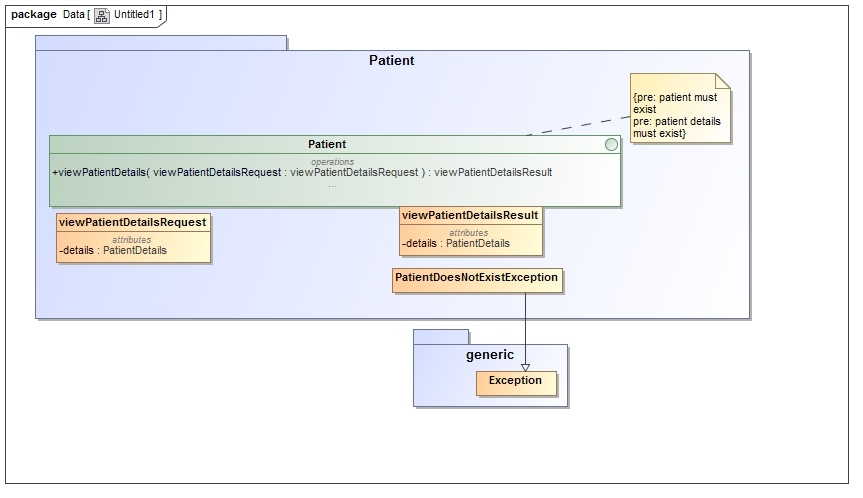
\includegraphics[width=1\linewidth]{./Graphics/1.jpg}
\subsubsection{Activity diagram:}
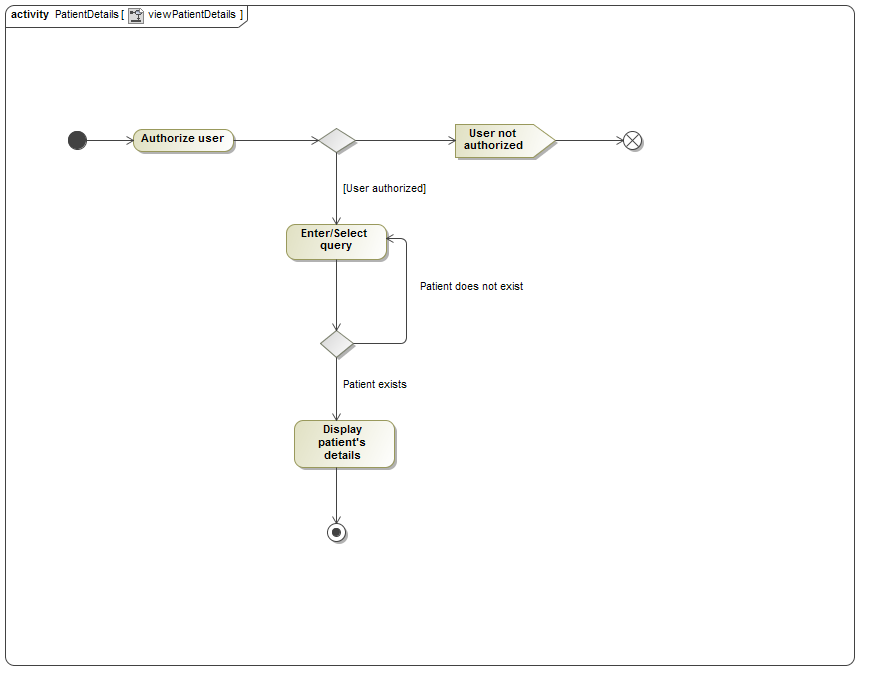
\includegraphics[width=1\linewidth]{./Graphics/viewPatientDetails.png}
%\left(

%Update patient details
\subsection{Update patient details}
\textbf{Description:}
This allows the administrator to update the details of a patient.
\subsubsection{Prioritization:}
Critical
\subsubsection{Conditions and Data Structures:}
\textbf{Pre-Conditions:}
	\begin{itemize}
	\item The user must be authorised to update the patient's details
	\item The patient must exist
	\item Patient's details must exist
	\end{itemize}
\textbf{Post-Conditions:}
	\begin{itemize}
	\item Patient's old details are updated
	\end{itemize}	
%\subsubsection{Required Functionality:} 
%\subsubsection{Process Specifications:}
\subsubsection{Service contract:}
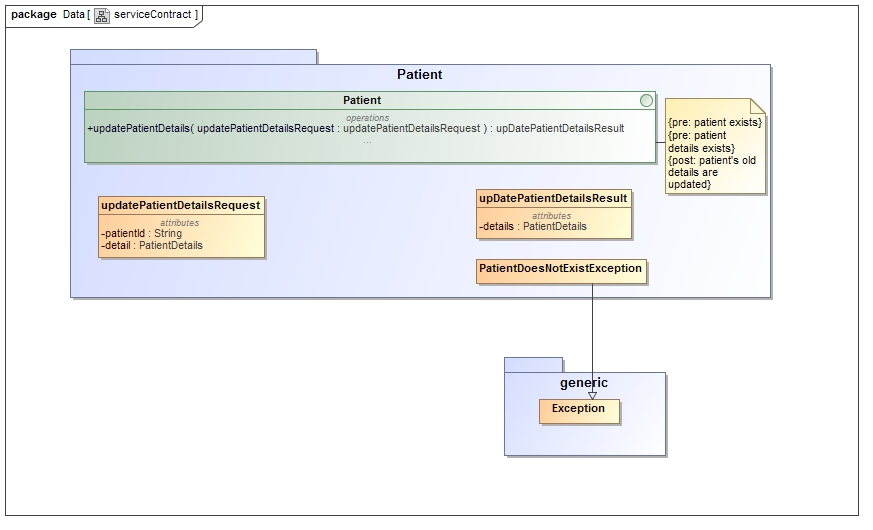
\includegraphics[width=1\linewidth]{./Graphics/2.jpg}
\subsubsection{Activity diagram:}
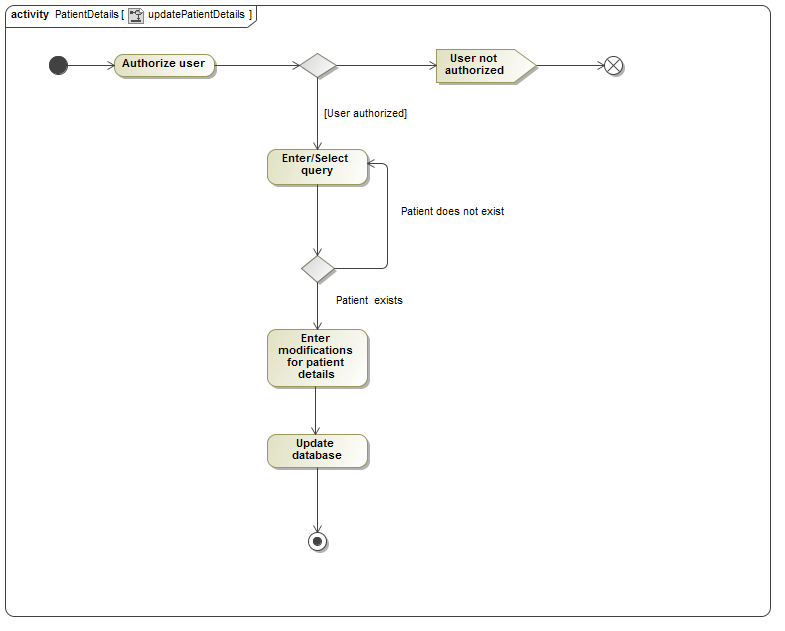
\includegraphics[width=1\linewidth]{./Graphics/updatePatientDetails.png}
%\left(

%Query All Patient Details
\subsection{Query All Patient Details}
\textbf{Description:}
This allows the administrator to query the database of patients; predefined functions are created.
\subsubsection{Prioritization:}
Critical
\subsubsection{Conditions and Data Structures:}
\textbf{Pre-Conditions:}
	\begin{itemize}
	\item The user must be authorised to query the database
	\item The patient must exist
	\item Query must be valid
	\end{itemize}
\textbf{Post-Conditions:}
	\begin{itemize}
	\item Query results are returned as a string
	\end{itemize}	
%\subsubsection{Required Functionality:} 
%\subsubsection{Process Specifications:}
\subsubsection{Service contract:}
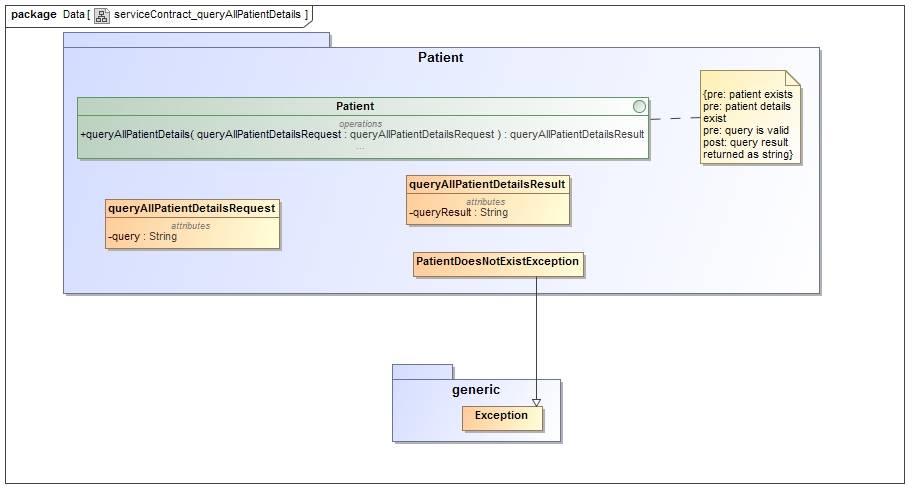
\includegraphics[width=1\linewidth]{./Graphics/3.jpg}
\subsubsection{Activity diagram:}
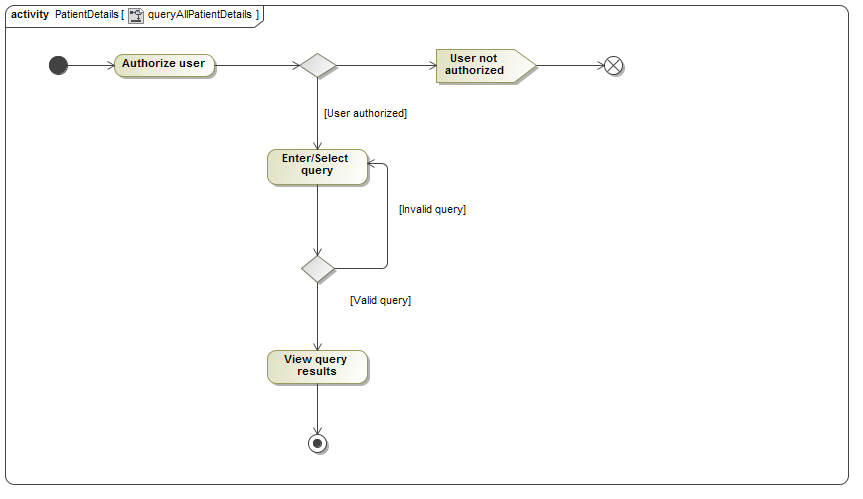
\includegraphics[width=1\linewidth]{./Graphics/queryAllPatientDetails.png}
%\left(
